% LaTeX source for textbook ``How to think like a computer scientist''
% Copyright (c)  2001  Allen B. Downey, Jeffrey Elkner, and Chris Meyers.

% Permission is granted to copy, distribute and/or modify this
% document under the terms of the GNU Free Documentation License,
% Version 1.1  or any later version published by the Free Software
% Foundation; with the Invariant Sections being "Contributor List",
% with no Front-Cover Texts, and with no Back-Cover Texts. A copy of
% the license is included in the section entitled "GNU Free
% Documentation License".

% This distribution includes a file named fdl.tex that contains the text
% of the GNU Free Documentation License.  If it is missing, you can obtain
% it from www.gnu.org or by writing to the Free Software Foundation,
% Inc., 59 Temple Place - Suite 330, Boston, MA 02111-1307, USA.

\chapter{Clases y objetos}
\index{clase}
\index{objeto}


\section{Tipos compuestos definidos por el usuario}
\label{point}
\index{tipo de datos compuestos}
\index{tipo de datos!compuesto}
\index{tipo de datos definido por el usuario}
\index{tipo de datos!definido por el usuario}
\index{constructor}

Una vez utilizados algunos de los tipos internos de Python, estamos listos
para crear un tipo definido por el usuario: el \texttt{Punto}.

Piense en el concepto de un punto matemático. En dos dimensiones, un punto
tiene dos números (coordenadas) que se tratan colectivamente como un solo
objeto. En notación matemática, los puntos suelen escribirse entre
paréntesis con una coma separando las coordenadas. Por ejemplo, $(0, 0)$
representa el origen, y $(x, y)$ representa el punto $x$ unidades a la
derecha e $y$ unidades hacia arriba desde el origen.

Una forma natural de representar un punto en Python es con dos valores en
punto flotante. La cuestión es, entonces, cómo agrupar esos dos valores en
un objeto compuesto. La solución rápida y burda es utilizar una lista o
tupla, y para algunas aplicaciones esa podría ser la mejor opción.

\index{coma flotante}

Una alternativa es que el usuario defina un nuevo tipo de dato compuesto, también
llamado una {\bf clase}. Esta aproximación exige un poco más de esfuerzo,
pero tiene algunas ventajas que pronto se harán evidentes.

Una definición de clase se parece a esto:

\beforeverb
\begin{verbatim}
class Punto:
  pass
\end{verbatim}
\afterverb
%
Las definiciones de clase pueden aparecer en cualquier lugar de un
programa, pero normalmente están al principio (tras las sentencias
\texttt{import}). Las reglas sintácticas de la definición de clases son
las mismas que para las otras sentencias compuestas. (ver la
Sección~\ref{alternative execution}).

Esta definición crea una nueva clase llamada \texttt{Punto}. La sentencia
{\bf pass} no tiene efectos; sólo es necesaria porque una sentencia
compuesta debe tener algo en su cuerpo.

Al crear la clase \texttt{Punto} hemos creado un nuevo tipo, que también
se llama \texttt{Punto}. Los miembros de este tipo se llaman {\bf instancias}
del tipo u {\bf objetos}. La creación de una nueva instancia se llama
{\bf instanciación}. Para instanciar un objeto \texttt{Punto} ejecutamos una
función que se llama (lo has adivinado) \texttt{Punto}:

\index{instancia!objeto}
\index{instancia de un objeto}
\index{instanciación}

\beforeverb
\begin{verbatim}
limpio = Punto()
\end{verbatim}
\afterverb
%
A la variable \texttt{limpio} se le asigna una referencia a un nuevo
objeto \texttt{Punto}. A una función como \texttt{Punto} que crea un
objeto nuevo se le llama {\bf constructor}.


\section{Atributos}
\index{atributos}

Podemos añadir nuevos datos a una instancia utilizando la notación de punto:

\beforeverb
\begin{verbatim}
>>> limpio.x = 3.0
>>> limpio.y = 4.0
\end{verbatim}
\afterverb
%
Esta sintaxis es similar a la sintaxis para seleccionar una variable de
un módulo, como \texttt{math.pi} o \texttt{string.uppercase}. En este caso,
sin embargo, estamos seleccionando un dato de una instancia. Estos datos
con nombre se denominan {\bf atributos}.

El diagrama de estados que sigue muestra el resultado de esas asignaciones:

\beforefig
\centerline{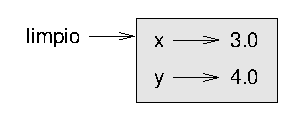
\includegraphics{illustrations/point.eps}}
\afterfig

La variable \texttt{limpio} apunta a un objeto Punto, que
contiene dos atributos. Cada atributo apunta a un número
en punto flotante.

Podemos leer el valor de un atributo utilizando la misma sintaxis:

\beforeverb
\begin{verbatim}
>>> print limpio.y
4.0
>>> x = limpio.x
>>> print x
3.0
\end{verbatim}
\afterverb
%
La expresión \texttt{limpio.x} significa, ``ve al objeto al que apunta \texttt{limpio}
y toma el valor de \texttt{x}''. En este caso, asignamos ese valor a una variable
llamada \texttt{x}. No hay conflicto entre la variable \texttt{x} y el atributo \texttt{x}.
El propósito de la notación punto es identificar de forma inequívoca a qué
variable se refiere el programador.

Se puede usar la notación punto como parte de cualquier expresión. Así, las
sentencias que siguen son correctas:

\beforeverb
\begin{verbatim}
print '(' + str(limpio.x) + ', ' + str(limpio.y) + ')'
distanciaAlCuadrado = limpio.x * limpio.x + 
                      limpio.y * limpio.y
\end{verbatim}
\afterverb
%
La primera línea presenta \texttt{(3.0, 4.0)}; la segunda línea calcula el valor 25.0.

Usted puede estar tentado a imprimir el propio valor de \texttt{limpio}:

\beforeverb
\begin{verbatim}
>>> print limpio
<__main__.Point instance at 80f8e70>
\end{verbatim}
\afterverb
%
El resultado indica que \texttt{limpio} es una instancia de la clase
\texttt{Punto} que se definió en \texttt{\_\_main\_\_}.  \texttt{80f8e70} es
el identificador único de este objeto, escrito en hexadecimal.
Probablemente ésta no es la manera más clara de mostrar un objeto
\texttt{Punto}. En breve veremos cómo cambiar esto.

\index{imprimir!objeto}

\section{Instancias como parámetro}
\index{instancia}
\index{parámetro}

Se puede pasar una instancia como parámetro de la forma habitual.
Por ejemplo:

\beforeverb
\begin{verbatim}
def imprimePunto(p):
  print '(' + str(p.x) + ', ' + str(p.y) + ')'
\end{verbatim}
\afterverb
%
\texttt{imprimePunto} acepta un punto como argumento y lo muestra
en el formato estándar de la matemática. Si llamas a \texttt{imprimePunto(limpio)}, el
resultado es \texttt{(3.0, 4.0)}.


\section{Mismidad}
\index{mismidad}

El significado de la palabra ``mismo'' parece totalmente claro hasta
que uno se detiene a pensarlo un poco y se da cuenta de que hay
algo más de lo que se supone comúnmente.

\index{ambigüedad}
\index{lenguaje natural}
\index{lenguaje}

Por ejemplo, si alguien dice ``Pepe y yo tenemos la misma moto'', lo que quiere decir
es que su moto y la de Pepe son de la misma marca y modelo, pero que son dos motos
distintas. Si dice ``Pepe y yo tenemos la misma madre'', quiere decir que su madre
y la de Pepe son la misma persona\footnote{No todas las lenguas tienen el mismo
problema. Por ejemplo, el alemán tiene palabras diferentes para los diferentes
tipos de identidad. ``Misma moto'' en este contexto sería ``gleiche Motorrad'' y ``misma
madre'' sería ``selbe Mutter''.}. Así que la idea de ``identidad'' es diferente según
el contexto.

Cuando uno habla de objetos, hay una ambigüedad parecida. Por ejemplo,
si dos \texttt{Puntos} son el mismo, ¿significa que contienen los mismos datos
(coordenadas) o que son de verdad el mismo objeto?

Para averiguar si dos referencias se refieren al mismo objeto, se utiliza el
operador \texttt{==}. Por ejemplo:

\beforeverb
\begin{verbatim}
>>> p1 = Punto()
>>> p1.x = 3
>>> p1.y = 4
>>> p2 = Punto()
>>> p2.x = 3
>>> p2.y = 4
>>> p1 == p2
False
\end{verbatim}
\afterverb
%
Aunque \texttt{p1} y \texttt{p2} contienen las mismas coordenadas, no son
el mismo objeto. Si asignamos \texttt{p1} a \texttt{p2}, las dos variables son
alias del mismo objeto:

\beforeverb
\begin{verbatim}
>>> p2 = p1
>>> p1 == p2
True
\end{verbatim}
\afterverb
%
Este tipo de igualdad se llama {\bf igualdad superficial}, porque sólo
compara las referencias, pero no el contenido de los objetos.

\index{igualdad}
\index{identidad}
\index{igualdad superficial}
\index{igualdad profunda}

Para comparar los contenidos de los objetos ({\bf igualdad profunda}) podemos
escribir una función llamada \texttt{mismoPunto}:

\beforeverb
\begin{verbatim}
def mismoPunto(p1, p2) :
  return (p1.x == p2.x) and (p1.y == p2.y)
\end{verbatim}
\afterverb
%
Si ahora creamos dos objetos diferentes que contienen los mismos datos
podremos usar \texttt{mismoPunto} para averiguar si representan el mismo punto:

\beforeverb
\begin{verbatim}
>>> p1 = Punto()
>>> p1.x = 3
>>> p1.y = 4
>>> p2 = Punto()
>>> p2.x = 3
>>> p2.y = 4
>>> mismoPunto(p1, p2)
True
\end{verbatim}
\afterverb
%
Por supuesto, si las dos variables apuntan al mismo objeto \texttt{mismoPunto}
devuelve verdadero.


\section{Rectángulos}
\label{embedded}
\index{rectángulo}

Digamos que queremos una clase que represente un rectángulo. La pregunta es,
¿qué información tenemos que proporcionar para definir un rectángulo? Para
simplificar las cosas, supongamos que el rectángulo está orientado vertical u
horizontalmente, nunca en diagonal.

Tenemos varias posibilidades: podemos señalar el centro del rectángulo
(dos coordenadas) y su tamaño (anchura y altura); o podemos señalar una de
las esquinas y el tamaño; o podemos señalar dos esquinas opuestas. Un modo
convencional es señalar la esquina superior izquierda del rectángulo y el tamaño.

De nuevo, definiremos una nueva clase:

\beforeverb
\begin{verbatim}
# ¡Prohibidos los acentos fuera de las cadenas!
class Rectangulo:	
  pass
\end{verbatim}
\afterverb
%
Y la instanciaremos:

\beforeverb
\begin{verbatim}
caja = Rectangulo()
caja.anchura = 100.0
caja.altura = 200.0
\end{verbatim}
\afterverb
%
Este código crea un nuevo objeto \texttt{Rectangulo} con dos atributos flotantes.
¡Para señalar la esquina superior izquierda podemos incrustar un objeto dentro de otro!

\beforeverb
\begin{verbatim}
caja.esquina = Punto()
caja.esquina.x = 0.0;
caja.esquina.y = 0.0;
\end{verbatim}
\afterverb
%
El operador punto compone. La expresión \texttt{caja.esquina.x} significa
"ve al objeto al que se refiere \texttt{caja} y selecciona el atributo llamado
\texttt{esquina}; entonces ve a ese objeto y selecciona el atributo llamado
\texttt{x}".

La figura muestra el estado de este objeto:

\beforefig
\centerline{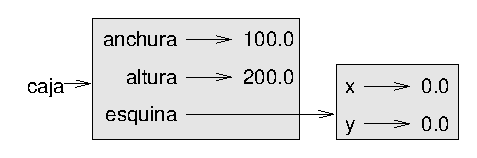
\includegraphics{illustrations/rectangle.eps}}
\afterfig


\section{Instancias como valores de retorno}
\index{instancia}
\index{valor de retorno}

Las funciones pueden devolver instancias. Por ejemplo, \texttt{encuentraCentro}
acepta un \texttt{Rectangulo} como argumento y devuelve un \texttt{Punto} que
contiene las coordenadas del centro del \texttt{Rectangulo}:

\beforeverb
\begin{verbatim}
def encuentraCentro(caja):
  p = Punto()
  p.x = caja.esquina.x + caja.anchura/2.0
  p.y = caja.esquina.y + caja.altura/2.0
  return p
\end{verbatim}
\afterverb
%
Para llamar a esta función, se pasa \texttt{caja} como argumento y se asigna el resultado
a una variable:

\beforeverb
\begin{verbatim}
>>> centro = encuentraCentro(caja)
>>> imprimePunto(centro)
(50.0, 100.0)
\end{verbatim}
\afterverb
%

\section{Los objetos son mutables}
\index{objeto!mutable}
\index{objeto mutable}

Podemos cambiar el estado de un objeto efectuando una asignación
sobre uno de sus atributos. Por ejemplo, para cambiar el tamaño de
un rectángulo sin cambiar su posición, podemos cambiar los valores de
\texttt{anchura} y \texttt{altura}:

\beforeverb
\begin{verbatim}
caja.anchura = caja.anchura + 50
caja.altura = caja.altura + 100
\end{verbatim}
\afterverb
%
Podemos encapsular este código en un método y generalizarlo
para agrandar el rectángulo en cualquier cantidad:

\index{encapsulamiento}
\index{generalización}

\beforeverb
\begin{verbatim}
def agrandarRect(caja, danchura, daltura) :
  caja.anchura = caja.anchura + danchura
  caja.altura = caja.altura + daltura
\end{verbatim}
\afterverb
%
Las variables \texttt{danchura} y \texttt{daltura} indican cuánto debe agrandarse
el rectángulo en cada dirección. Invocar este método tiene el efecto de
modificar el \texttt{Rectangulo} que se pasa como argumento.

Por ejemplo, podemos crear un nuevo \texttt{Rectangulo} llamado \texttt{b}
y pasárselo a la función \texttt{agrandarRect}:

\beforeverb
\begin{verbatim}
>>> b = Rectangulo()
>>> b.anchura = 100.0
>>> b.altura = 200.0
>>> b.esquina = Punto()
>>> b.esquina.x = 0.0;
>>> b.esquina.y = 0.0;
>>> agrandarRect(b, 50, 100)
\end{verbatim}
\afterverb
%
Mientras \texttt{agrandarRect} se está ejecutando, el parámetro \texttt{caja} es un
alias de \texttt{b}. Cualquier cambio que se hagas a \texttt{caja} afectará también a
\texttt{b}.


\section{Copiado}
\index{uso de alias}
\index{copiado}
\index{módulo copy}
\index{módulo!copy}

El uso de un alias puede hacer que un programa sea difícil de leer,
porque los cambios hechos en un lugar pueden tener efectos inesperados
en otro lugar. Es difícil estar al tanto de todas las variables que 
pueden apuntar a un objeto dado.

Copiar un objeto es, muchas veces, una alternativa a la creación de un alias.
El módulo \texttt{copy} contiene una función llamada \texttt{copy} que puede
duplicar cualquier objeto:

\beforeverb
\begin{verbatim}
>>> import copy
>>> p1 = Punto()
>>> p1.x = 3
>>> p1.y = 4
>>> p2 = copy.copy(p1)
>>> p1 == p2
False
>>> mismoPunto(p1, p2)
True
\end{verbatim}
\afterverb
%
Una vez que hemos importado el módulo \texttt{copy}, podemos usar el método \texttt{copy}
para hacer un nuevo \texttt{Punto}.  \texttt{p1} y \texttt{p2} no son el mismo punto, pero
contienen los mismos datos.

Para copiar un objeto simple como un \texttt{Punto}, que no contiene objetos incrustados,
\texttt{copy} es suficiente. Esto se llama {\bf copiado superficial}.

Para algo como un \texttt{Rectangulo}, que contiene una referencia a un 
\texttt{Punto}, \texttt{copy} no lo hace del todo bien. Copia la referencia al objeto
\texttt{Punto}, de modo que tanto el \texttt{Rectangulo} viejo como el nuevo apuntan a
un único \texttt{Punto}.

Si creamos una caja, \texttt{b1}, de la forma habitual y entonces hacemos una
copia, \texttt{b2}, usando \texttt{copy}, el diagrama de estados resultante se ve
así:

\beforefig
\centerline{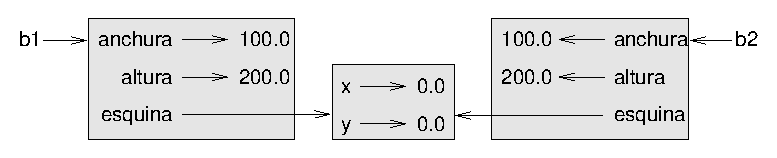
\includegraphics{illustrations/rectangle2.eps}}
\afterfig

Es casi seguro que esto no es lo que queremos. En este caso, la invocación
de \texttt{agrandaRect} sobre uno de los \texttt{Rectangulo}s no afectaría al otro,
¡pero la invocación de \texttt{mueveRect} sobre cualquiera afectaría a ambos!
Este comportamiento es confuso y propicia los errores.

Afortunadamente, el módulo \texttt{copy} contiene un método llamado {\tt
deepcopy} que copia no sólo el objeto, sino también cualesquiera objetos
incrustados en él. No lo sorprenderá saber que esta operación se llama {\bf
copia profunda} (deep copy).

\beforeverb
\begin{verbatim}
>>> b2 = copy.deepcopy(b1)
\end{verbatim}
\afterverb
%
Ahora \texttt{b1} y \texttt{b2} son objetos totalmente independientes.

Podemos usar \texttt{deepcopy} para reescribir \texttt{agrandaRect} de modo que
en lugar de modificar un \texttt{Rectangulo} existente, cree un nuevo
\texttt{Rectangulo} que tiene la misma localización que el viejo pero nuevas
dimensiones:

\beforeverb
\begin{verbatim}
def agrandaRect(caja, danchura, daltura) :
  import copy
  nuevaCaja = copy.deepcopy(caja)
  nuevaCaja.anchura = nuevaCaja.anchura + danchura
  nuevaCaja.altura = nuevaCaja.altura + daltura
  return nuevaCaja
\end{verbatim}
\afterverb
%

\section{Glosario}

\begin{description}

\item[Clase:] tipo compuesto definido por el usuario. También se puede pensar en una
clase como una plantilla para los objetos que son instancias de la misma.

\item[Instanciar:] Crear una instancia de una clase.

\item[Instancia:] objeto que pertenece a una clase.

\item[Objeto:] tipo de dato compuesto que suele usarse para representar
una cosa o concepto del mundo real.

\item[Constructor:] método usado para crear nuevos objetos.

\item[Atributo:] uno de los elementos de datos con nombre que
constituyen una instancia.

\item[Igualdad superficial:] igualdad de referencias, o dos referencias
que apuntan al mismo objeto.

\item[Igualdad profunda:] igualdad de valores, o dos referencias que apuntan
a objetos que tienen el mismo valor.

\item[Copia superficial:] copiar el contenido de un objeto, incluyendo
cualquier referencia a objetos incrustados; implementada por la función \texttt{copy}
del módulo \texttt{copy}.

\item[Copia profunda:] copiar el contenido de un objeto así como cualesquiera
objetos incrustados, y los incrustados en estos, y así sucesivamente. Está implementada 
en la función \texttt{deepcopy} del módulo \texttt{copy}.

\index{clase}
\index{instanciar}
\index{instancia}
\index{objeto}
\index{constructor}
\index{atributo}
\index{igualdad superficial}
\index{igualdad profunda}
\index{copia superficial}
\index{copia profunda}

\end{description}

\section{Ejercicios}

\begin{enumerate}
\item  Cree e imprima un objeto \texttt{Punto} y luego use
\texttt{id} para imprimir el identificador único del objeto. Traduzca 
el número hexadecimal a decimal y asegúrese de que coincidan.

\item  Reescriba la función \texttt{distancia} de la
Sección~\ref{program development} de forma que acepte dos \texttt{Puntos} como
parámetros en lugar de cuatro números.

\item Reescriba \texttt{mueveRect} de modo que cree y devuelva
un nuevo \texttt{Rectangulo} en lugar de modificar el viejo.

\item Investigue la documentación del módulo Turtle de Python. 
Escriba una función que dibuje un rectángulo con la tortuga.

\item Escriba un programa que dibuje dos tortugas haciendo un movimiento circular 
permanente.Pista: Piense en como intercalar los movimientos de las dos tortugas.

\item Escriba una función llamada \texttt{mueveRect} que tome
un \texttt{Rectangulo} y dos parámetros llamados \texttt{dx} y \texttt{dy}. 
Tiene que cambiar la posición del rectángulo añadiendo en la  \texttt{esquina}: 
\texttt{dx} a la coordenada \texttt{x}  y  \texttt{dy} a la coordenada \texttt{y}.

\end{enumerate}
